% =============================================================================
% FYP Final Progress Review -- SkinCare AI
% Course: CMP6200 / DIG6200
% Target: 1500-word ceiling. Body target ~1480. See comment block per section.
% Build:  pdflatex fyp_progress_review.tex   (run twice if needed)
% Count:  texcount fyp_progress_review.tex  (optional)
% =============================================================================

\documentclass[11pt,a4paper]{article}

\usepackage[margin=1.15in]{geometry}
\usepackage[T1]{fontenc}
\usepackage[utf8]{inputenc}
\usepackage{lmodern}
\usepackage{microtype}
\usepackage{parskip}
\usepackage{titlesec}
\usepackage{enumitem}
\usepackage{graphicx}
\usepackage{booktabs}
\usepackage{array}
\usepackage{tabularx}
\usepackage{multirow}
\usepackage{caption}
\usepackage{hyperref}
\usepackage{tikz}
\usetikzlibrary{shapes.geometric, arrows.meta, positioning, fit, backgrounds, calc}

\hypersetup{
  colorlinks=true,
  linkcolor=black,
  urlcolor=black,
  citecolor=black,
  pdftitle={FYP Final Progress Review -- SkinCare AI},
  pdfauthor={Krishu Karki}
}

% --- Visual tweaks ----------------------------------------------------------
% Each \section begins on its own page.
\let\oldsection\section
\renewcommand{\section}{\clearpage\oldsection}
\titleformat{\section}{\large\bfseries}{\thesection.0}{0.6em}{}
\titleformat{\subsection}{\normalsize\bfseries}{\thesubsection}{0.6em}{}
\titlespacing*{\section}{0pt}{1.2em}{0.4em}
\titlespacing*{\subsection}{0pt}{0.9em}{0.3em}
\setlist{nosep,leftmargin=1.2em}

\captionsetup{font=small,labelfont=bf,skip=4pt}

% -----------------------------------------------------------------------------
\newcommand{\ProjectTitle}{SkinCare AI: AI-Powered Skin Condition, Skin-Type Detection and Product Recommendation for Nepal}
\newcommand{\StudentName}{Krishu Karki}
\newcommand{\StudentID}{23189624}
\newcommand{\CourseTitle}{Individual Final Year Project}
\newcommand{\Supervisor}{Praskash Gautam}
\newcommand{\LastReview}{14th June}
\newcommand{\ThisReview}{03 Sep 2026}

\title{\ProjectTitle}
\author{\StudentName \;--\; ID: \StudentID}
\date{}

\begin{document}

% =============================================================================
% Cover block
% =============================================================================
\begin{center}
  {\small CMP6200 / DIG6200 --- Individual Undergraduate Project (FYP)}\\[0.2em]
  {\Large\bfseries Final Progress Review}\\[0.4em]
  \rule{0.85\linewidth}{0.4pt}\\[0.4em]
  {\large\bfseries \ProjectTitle}\\[0.6em]
  \begin{tabular}{@{}r@{\hspace{0.6em}}l@{}}
    \textbf{Student Name:}     & \StudentName \\
    \textbf{Student ID:}       & \StudentID \\
    \textbf{Course:}           & \CourseTitle \\
    \textbf{Supervisor:}       & \Supervisor \\
    \textbf{Reporting Period:} & \LastReview{} to \ThisReview \\
  \end{tabular}
\end{center}
\vspace{0.4em}

% =============================================================================
% Word budget: hard cap 1500. Per-section target in comments.
%   S1 = 200, S2.1 = 480, S2.2 = 480, S3.1 = 220, S3.2 = 180  --> ~1560
%   tighten to land 1480-1500. Tables/figures count as ~30 words each.
% =============================================================================

% -----------------------------------------------------------------------------
% 1.0  Progress to Date -- Summary  (target: ~200 words)
% -----------------------------------------------------------------------------
\section{Progress to Date --- Summary}

The project is in the advanced prototyping and pre-evaluation phase and
is broadly on track. Since the last review, four artefacts have moved
from partial prototypes to working end-to-end implementations: the data
enrichment pipeline, the multi-task image model, the rule-based
recommendation engine, and the user-facing surfaces. Product data from
three Nepali e-commerce sources (\emph{ForEveryNG}, \emph{Jeevee}, and
\emph{Oriflame}) has been merged, NLP-enriched, and fuzzy-deduplicated
into a single canonical catalogue. A shared-backbone EfficientNetB0 has
been trained as a multi-task model: a seven-class condition head
(\emph{Acne}, \emph{Carcinoma}, \emph{Dark Spot}, \emph{Eczema},
\emph{Keratosis}, \emph{Milia}, \emph{Rosacea}) plus a three-class
skin-type head (\emph{dry}, \emph{normal}, \emph{oily}) using
sample-masked cross-entropy losses. The recommendation engine now takes
both condition and skin type as input, and an optional on-device small
language model layer (Qwen2.5-1.5B-Instruct via HuggingFace) reranks
the deterministic shortlist and writes a personalised AM/PM routine.
Two surfaces expose the flow: a Streamlit app and a FastAPI backend.
The most significant development of this period is the move from a
single-task five-class detector to the present multi-task
seven-condition + three-skin-type design, paired with a guardrailed
SLM rerank; this re-scoping is reflected across the model, the
recommender defaults, the medical gate, and the API contracts, and has
tightened the artefact's behaviour in real-world conditions.

% -----------------------------------------------------------------------------
% 2.0  Artefact Design and Development  (core section)
% -----------------------------------------------------------------------------
\section{Artefact Design and Development}

This section is the core of the report: it describes what the artefact
is, why it has been built the way it has, and what has been learned
from working on it. The implementation is presented first as evidence;
the analysis follows as interpretation.

% --- 2.1  Implementation and Current State  (target: ~480 words) ------------
\subsection{Implementation and Current State}

The system is organised as five tiers plus an optional guardrailed
rerank layer, summarised in \autoref{fig:architecture},
\autoref{fig:workflow} and \autoref{tab:modules}. The data tier reads
raw product catalogues from
the three Nepali retailers, joins them on brand, name, price and
ingredients, NLP-tags each row with category, ingredients, skin types
and concerns, then fuzzy-deduplicates at an 85\% similarity threshold
using rapidfuzz, and emits a single unified catalogue. The model tier
loads condition and skin-type image folders, tags each per-task
pipeline as a two-key dictionary with an ignore label for the head
that does not own the sample, and interleaves them into a single
training stream with the skin-type side over-sampled to compensate for
its much smaller size. The multi-task model shares an EfficientNetB0
backbone, a 256-dimensional shared dense trunk, and two softmax heads;
the custom training step applies masked sparse cross-entropy per head.
Two-phase training first freezes the base at learning rate \(10^{-3}\)
for 20 epochs, then unfreezes the top 30 base layers at learning rate
\(10^{-5}\) for 15 epochs, with early stopping on the condition
validation accuracy and learning-rate reduction on plateau. The
recommendation tier takes a (condition, skin-type) pair and runs a
rule engine that maps the condition to a hand-written policy,
filters the catalogue by recommended categories, then ranks with a
weighted sum: ingredient match 0.40, rating 0.25, reviews 0.20,
availability 0.10, discount 0.05, plus a skin-type block at 0.25
when a skin type is known. The presentation tier is a Streamlit app
and a FastAPI backend, both of which call the same analyse entry
point. A guardrailed SLM layer loads Qwen2.5-1.5B-Instruct on CPU in
bfloat16 (with a 0.5B fallback), receives only the deterministic
shortlist, and any product ID it invents is dropped in code. Carcinoma
bypasses both the engine and the SLM and returns a dermatologist-only
response. The seven condition classes and their attached policies are
listed in \autoref{tab:conditions}, and the Streamlit surface is shown
schematically in \autoref{fig:ui}. The end-to-end pipeline is
orchestrated by a single command-line entry point that supports
data, train, inference and all steps, and is tracked in a single
\emph{git} repository with conventional commits on \emph{main}.

% ---- Table 1: Module responsibilities --------------------------------------
\begin{table}[!ht]
  \centering
  \caption{Module responsibilities across the five tiers of the artefact.}
  \label{tab:modules}
  \begin{tabularx}{\linewidth}{@{}p{2.4cm} X p{4.0cm}@{}}
    \toprule
    \textbf{Tier} & \textbf{Responsibility} & \textbf{Where it lives} \\
    \midrule
    Data       & Merge, NLP-enrich, fuzzy-dedup three Nepali catalogues.            & Data pipeline \\
    Model      & Multi-task EfficientNetB0 (condition + skin type), two-phase training. & Model package \\
    Recommend  & Rule-based candidates + weighted scoring + skin-type match.        & Recommendation package \\
    Present    & Streamlit UI and FastAPI routes for the same analysis flow.        & App + backend \\
    SLM        & Optional Qwen2.5-1.5B rerank of the deterministic shortlist, with shortlist validation. & SLM package \\
    \bottomrule
  \end{tabularx}
\end{table}

% ---- Figure 1: Architecture diagram (TikZ) ----------------------------------
\begin{figure}[!ht]
  \centering
  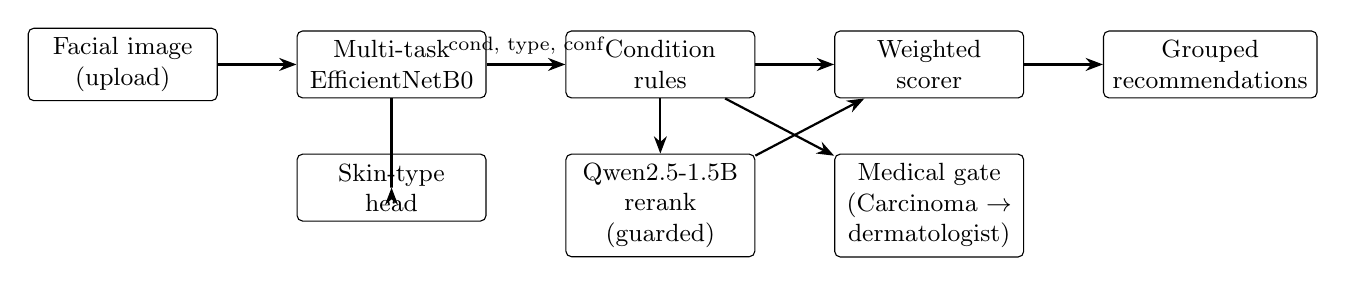
\begin{tikzpicture}[
      node distance=0.7cm and 1.0cm,
      box/.style={rectangle, draw=black, rounded corners=2pt,
                  minimum width=2.4cm, minimum height=0.85cm, align=center,
                  font=\small},
      io/.style={box},
      arr/.style={-{Stealth[length=2.2mm]}, thick}
    ]
    \node[io]  (img)                 {Facial image\\(upload)};
    \node[box, right=of img]  (model) {Multi-task\\EfficientNetB0};
    \node[box, right=of model](rules) {Condition\\rules};
    \node[box, right=of rules](score) {Weighted\\scorer};
    \node[io,  right=of score](out)   {Grouped\\recommendations};

    \node[box, below=of model]  (type) {Skin-type\\head};
    \node[box, below=of rules]  (slm)  {Qwen2.5-1.5B\\rerank\\(guarded)};
    \node[box, below=of score]  (med)  {Medical gate\\(Carcinoma $\rightarrow$ \\dermatologist)};

    \draw[arr] (img)   -- (model);
    \draw[arr] (model) |- (type);
    \draw[arr] (model) -- node[above]{\scriptsize cond, type, conf} (rules);
    \draw[arr] (rules) -- (score);
    \draw[arr] (score) -- (out);
    \draw[arr] (rules) -- (slm);
    \draw[arr] (slm)  -- (score);
    \draw[arr] (rules) -- (med);
  \end{tikzpicture}
  \caption{Five-tier architecture: image $\rightarrow$ multi-task
           EfficientNetB0 $\rightarrow$ condition rules $\rightarrow$
           weighted scorer $\rightarrow$ grouped output, with the
           guarded Qwen2.5-1.5B rerank and a medical short-circuit.}
  \label{fig:architecture}
\end{figure}

% ---- End-to-end workflow figure (mirrors skin_care_ai_workflow.drawio) -----
\begin{figure}[!ht]
  \centering
  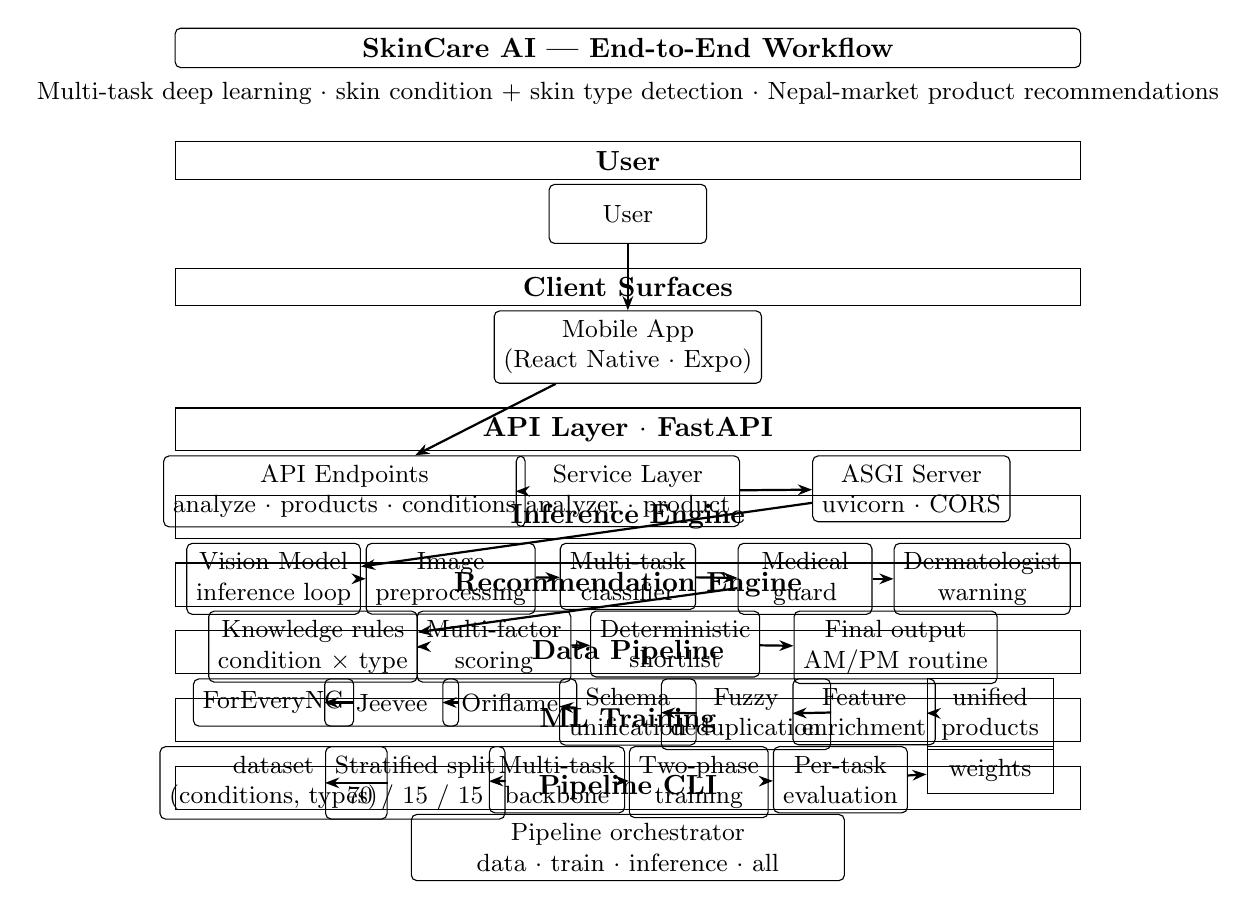
\begin{tikzpicture}[
      font=\small,
      node distance=0.55cm and 0.7cm,
      head/.style={rectangle, draw=black, rounded corners=2pt,
                   minimum width=11.5cm, minimum height=0.5cm, align=center,
                   font=\bfseries},
      tier/.style={rectangle, draw=black, minimum width=11.5cm,
                   minimum height=0.35cm, align=center, font=\bfseries},
      box/.style={rectangle, draw=black, rounded corners=2pt,
                  minimum width=2.0cm, minimum height=0.75cm, align=center},
      sub/.style={box, minimum width=1.7cm, minimum height=0.6cm},
      cyl/.style={cylinder, draw=black, shape border rotate=90, aspect=0.3,
                  minimum height=0.7cm, minimum width=1.8cm, align=center},
      doc/.style={rectangle, draw=black, minimum width=1.6cm,
                  minimum height=0.6cm, align=center},
      arr/.style={-{Stealth[length=1.8mm]}, thick}
    ]
    % Header
    \node[head] (title) {SkinCare AI --- End-to-End Workflow};
    \node[below=0.05cm of title] (sub) {Multi-task deep learning $\cdot$ skin condition + skin type detection $\cdot$ Nepal-market product recommendations};

    % Row 1: User
    \node[tier, below=0.35cm of sub] (r1) {User};
    \node[box, below=0.05cm of r1] (user) {User};

    % Row 2: Client
    \node[tier, below=0.30cm of user] (r2) {Client Surfaces};
    \node[box, below=0.05cm of r2] (mob) {Mobile App\\(React Native $\cdot$ Expo)};

    % Row 3: API
    \node[tier, below=0.30cm of mob] (r3) {API Layer $\cdot$ FastAPI};
    \node[sub, below=0.05cm of r3, xshift=-3.6cm] (api1) {API Endpoints\\analyze $\cdot$ products $\cdot$ conditions};
    \node[sub, below=0.05cm of r3] (api2) {Service Layer\\analyzer $\cdot$ product};
    \node[sub, below=0.05cm of r3, xshift=3.6cm] (api3) {ASGI Server\\uvicorn $\cdot$ CORS};

    % Row 4: Inference
    \node[tier, below=0.55cm of r3] (r4) {Inference Engine};
    \node[sub, below=0.05cm of r4, xshift=-4.5cm] (vis) {Vision Model\\inference loop};
    \node[sub, below=0.05cm of r4, xshift=-2.25cm] (pre) {Image\\preprocessing};
    \node[sub, below=0.05cm of r4] (cls) {Multi-task\\classifier};
    \node[sub, below=0.05cm of r4, xshift=2.25cm] (grd) {Medical\\guard};
    \node[sub, below=0.05cm of r4, xshift=4.5cm] (wrn) {Dermatologist\\warning};

    % Row 5: Recommendation
    \node[tier, below=0.30cm of r4] (r5) {Recommendation Engine};
    \node[sub, below=0.05cm of r5, xshift=-4.0cm] (rul) {Knowledge rules\\condition $\times$ type};
    \node[sub, below=0.05cm of r5, xshift=-1.7cm] (scr) {Multi-factor\\scoring};
    \node[sub, below=0.05cm of r5, xshift=0.6cm] (sho) {Deterministic\\shortlist};
    \node[sub, below=0.05cm of r5, xshift=3.4cm] (rec) {Final output\\AM/PM routine};

    % Row 6: Data
    \node[tier, below=0.30cm of r5] (r6) {Data Pipeline};
    \node[sub, below=0.05cm of r6, xshift=-4.5cm] (d1) {ForEveryNG};
    \node[sub, below=0.05cm of r6, xshift=-3.0cm] (d2) {Jeevee};
    \node[sub, below=0.05cm of r6, xshift=-1.5cm] (d3) {Oriflame};
    \node[sub, below=0.05cm of r6] (mrg) {Schema\\unification};
    \node[sub, below=0.05cm of r6, xshift=1.5cm] (ded) {Fuzzy\\deduplication};
    \node[sub, below=0.05cm of r6, xshift=3.0cm] (enr) {Feature\\enrichment};
    \node[doc, below=0.05cm of r6, xshift=4.6cm] (unf) {unified\\products};

    % Row 7: ML
    \node[tier, below=0.30cm of r6] (r7) {ML Training};
    \node[sub, below=0.05cm of r7, xshift=-4.5cm] (img) {dataset\\(conditions, types)};
    \node[sub, below=0.05cm of r7, xshift=-2.7cm] (spl) {Stratified split\\70 / 15 / 15};
    \node[sub, below=0.05cm of r7, xshift=-0.9cm] (mdl) {Multi-task\\backbone};
    \node[sub, below=0.05cm of r7, xshift=0.9cm] (trn) {Two-phase\\training};
    \node[sub, below=0.05cm of r7, xshift=2.7cm] (evl) {Per-task\\evaluation};
    \node[doc, below=0.05cm of r7, xshift=4.6cm] (wht) {weights};

    % Row 8: CLI
    \node[tier, below=0.30cm of r7] (r8) {Pipeline CLI};
    \node[box, below=0.05cm of r8, minimum width=5.5cm] (cli) {Pipeline orchestrator\\data $\cdot$ train $\cdot$ inference $\cdot$ all};

    % Arrows: vertical spine
    \draw[arr] (user) -- (mob);
    \draw[arr] (mob) -- (api1);
    \draw[arr] (api1) -- (api2);
    \draw[arr] (api2) -- (api3);
    \draw[arr] (api3) -- (vis);
    \draw[arr] (vis) -- (pre);
    \draw[arr] (pre) -- (cls);
    \draw[arr] (cls) -- (grd);
    \draw[arr] (grd) -- (wrn);
    \draw[arr] (grd) -- (rul);
    \draw[arr] (rul) -- (scr);
    \draw[arr] (scr) -- (sho);
    \draw[arr] (sho) -- (rec);
    \draw[arr] (d1) -- (d2);
    \draw[arr] (d2) -- (d3);
    \draw[arr] (d3) -- (mrg);
    \draw[arr] (mrg) -- (ded);
    \draw[arr] (ded) -- (enr);
    \draw[arr] (enr) -- (unf);
    \draw[arr] (img) -- (spl);
    \draw[arr] (spl) -- (mdl);
    \draw[arr] (mdl) -- (trn);
    \draw[arr] (trn) -- (evl);
    \draw[arr] (evl) -- (wht);
  \end{tikzpicture}
  \caption{End-to-end workflow of the artefact, rendered from the
           project diagram. The same five tiers --- client surface,
           API layer, inference engine, recommendation engine, and data
           pipeline --- appear in the Streamlit and FastAPI surfaces,
           and the multi-task model is shared by the inference and
           training paths.}
  \label{fig:workflow}
\end{figure}

% ---- Table 2: Condition classes & recommender policy ------------------------
\begin{table}[!ht]
  \centering
  \caption{Condition classes recognised by the model and the recommender
           policy attached to each.}
  \label{tab:conditions}
  \begin{tabularx}{\linewidth}{@{}p{2.4cm} p{2.0cm} X p{2.6cm}@{}}
    \toprule
    \textbf{Condition} & \textbf{Flag} & \textbf{Recommender policy} & \textbf{Disclaimer} \\
    \midrule
    Acne        & cosmetic & Cleanser + serum + moisturiser; salicylic, niacinamide. & Routine advice. \\
    Carcinoma   & medical  & No product recommendations; dermatologist referral.        & See a dermatologist. \\
    Dark Spot   & cosmetic & Serum + sunscreen; vitamin C, niacinamide, azelaic.       & Routine advice. \\
    Eczema      & medical  & Gentle cleanser + ceramide moisturiser.                   & See a dermatologist. \\
    Keratosis   & medical  & AHA/BHA exfoliant + urea moisturiser + sunscreen.         & See a dermatologist. \\
    Milia       & cosmetic & Light moisturiser; retinol serum (PM).                    & Avoid extraction. \\
    Rosacea     & cosmetic & Fragrance-free moisturiser + mineral sunscreen.           & Routine advice. \\
    \bottomrule
  \end{tabularx}
\end{table}

% ---- Figure 2: Streamlit UI placeholder ------------------------------------
\begin{figure}[!ht]
  \centering
  \fbox{\begin{minipage}[c][4.6cm][c]{0.86\linewidth}
    \centering
    \textit{\small [Screenshot placeholder] Streamlit app: image upload
              (left column) and detection result with confidence bar,
              grouped product cards, and disclaimer banner (right column).}
  \end{minipage}}
  \caption{Streamlit front end: upload + analyse, then read the ranked
           recommendations, the SLM explanation (when enabled), and the
           disclaimer.}
  \label{fig:ui}
\end{figure}

% --- 2.2  Analysis and Reflection  (target: ~480 words) ----------------------
\subsection{Analysis and Reflection}

The current finding is that the detection-to-recommendation path is
end-to-end functional, the recommendation engine is unit-runnable
across all seven conditions and all three skin types, and the SLM
layer is unit-testable without the model weights; the trained weights
file is not present in this checkout, so the held-out test pass and
the 5-fold cross-validation on the skin-type head are scheduled as the
next evaluation steps rather than reported here. Three design choices
are worth reflecting on. First, the multi-task head with sample-masked
losses was a response to a concrete data problem: the skin-type set
has roughly 112 images while the condition set is much larger, so a
naive joint softmax would be dominated by conditions. Tagging every
batch as a two-key dictionary with an ignore label for the non-owning
head, and over-sampling the type stream, lets a single backbone learn
both tasks without one drowning the other. Second, the SLM was
deliberately framed as a rerank over a deterministic shortlist rather
than a free-form generator: it sees the candidate list, must reply in
JSON, and any product ID it names that is not in the shortlist is
dropped in code. Carcinoma bypasses the SLM entirely. This
guardrail-first design is what makes the SLM safe to ship. Third, the
scoring weights lean hard on ingredient match (0.40), then rating and
reviews, with skin type as a swap-in block (0.25) when known; this
implicitly penalises products with empty ingredient lists even when
they are frequent in the catalogue.

A specific instance where the design had to be revised is the move
from a single-task five-class detector to the present multi-task
seven-condition + three-skin-type model with an SLM rerank layer
(mid-project, recorded in the version history). The original plan
treated skin type as a
separate post-hoc question and skin condition as a single label, but
preliminary tests showed that skin type materially changes which
products are sensible (a rich ceramide cream is not the same pick
for oily vs dry skin), and that the explanation layer was much more
useful when grounded in a verified shortlist. \autoref{tab:revisions}
records the principal design revisions made during the project so
far.

\begin{table}[!ht]
  \centering
  \caption{Principal design revisions since the interim review.}
  \label{tab:revisions}
  \begin{tabularx}{\linewidth}{@{}p{1.8cm} p{4.0cm} X@{}}
    \toprule
    \textbf{Stage} & \textbf{Original design} & \textbf{What changed and why} \\
    \midrule
    Classes   & Single-task five conditions.        & Multi-task seven conditions + three skin types with masked losses (mid-project revision). \\
    Scoring   & Keyword match on ingredients.       & Weighted scorer: ingredient, rating, reviews, availability, discount, plus skin-type block. \\
    Chatbot   & Free-form follow-up.                 & Replaced with a guarded SLM rerank on the deterministic shortlist; medical conditions bypass. \\
    Backend   & Streamlit only.                      & Added FastAPI service for programmatic access. \\
    UI        & Tabs for detection and products.     & Single page with two columns and inline SLM panel to reduce navigation. \\
    \bottomrule
  \end{tabularx}
\end{table}

Compared with the original problem statement ---
\emph{``help Nepali consumers identify common facial skin conditions
and find suitable, locally available products''} --- the artefact now
addresses every clause: identification (multi-task EfficientNetB0),
personalisation (skin-type head + skin-type-aware scoring), product
linkage (recommender over Nepali sources), and usability (Streamlit
plus FastAPI plus SLM explanation). The biggest shift in my own
understanding is that an AI artefact in this domain is less a
classifier and more a triage and personalisation surface: the
recommender, the skin-type head, and the medical gate carry as much
weight as the model's accuracy. UAT will test that hypothesis
directly.


% -----------------------------------------------------------------------------
% 3.0  Updated Planning for Project Completion
% -----------------------------------------------------------------------------
\section{Updated Planning for Project Completion}

% --- 3.1  Remaining Tasks  (target: ~220 words) -----------------------------
\subsection{Remaining Tasks}

The remaining work, ordered by priority and dependency, is summarised
in \autoref{tab:tasks} and expanded below.

\begin{table}[!ht]
  \centering
  \caption{Remaining tasks ordered by priority, with effort and dependency.}
  \label{tab:tasks}
  \begin{tabularx}{\linewidth}{@{}p{0.6cm} X p{1.4cm} p{2.6cm}@{}}
    \toprule
    \textbf{\#} & \textbf{Task} & \textbf{Effort} & \textbf{Depends on} \\
    \midrule
    1 & Train the multi-task model on the full dataset and produce weights. & 2 days  & Dataset ready. \\
    2 & Run the multi-task evaluation on the test split and 5-fold CV on the skin-type head. & 2 days  & Task 1. \\
    3 & User acceptance testing with 8--10 Nepali users. & 1 week  & Tasks 1--2. \\
    4 & Draft Discussion and Conclusion chapters.       & 1 week  & Tasks 1--3. \\
    5 & Buffer for deployment / model regressions.       & 1 week  & --- \\
    6 & Viva preparation: rehearsal, slides, demo script. & 3 days  & Report drafted. \\
    \bottomrule
  \end{tabularx}
\end{table}

Training and evaluation are the highest-priority tasks because the
Evaluation chapter depends on them, and the Discussion chapter needs
real numbers --- not just the design story --- to discuss trade-offs
honestly. The buffer week absorbs unexpected regressions in the
Streamlit deployment or the model file; it is deliberately not
scheduled for new features, in line with the proposal's risk plan.

% --- 3.2  Draft Outline of Final Report  (target: ~180 words) ----------------
\subsection{Draft Outline of Final Report}

The final dissertation will follow a six-chapter structure, tailored
to a software-engineering FYP with an embedded empirical study. The
chapter map is shown in \autoref{tab:outline}.

\begin{table}[!ht]
  \centering
  \caption{Chapter outline of the final dissertation.}
  \label{tab:outline}
  \begin{tabularx}{\linewidth}{@{}p{0.7cm} p{3.4cm} X@{}}
    \toprule
    \textbf{Ch.} & \textbf{Title} & \textbf{Core content} \\
    \midrule
    1 & Introduction       & Motivation, problem statement, aims, scope, Nepal-market context. \\
    2 & Literature Review  & Skin-lesion classification, e-commerce recommenders, on-device LLMs. \\
    3 & Methodology        & Datasets, enrichment pipeline, multi-task model, recommender design, evaluation protocol. \\
    4 & Implementation     & Architecture, multi-task training, scoring engine, Streamlit, FastAPI, SLM rerank. \\
    5 & Evaluation         & Per-task metrics, 5-fold CV on the skin-type head, UAT findings, recommender relevance, medical-gate behaviour. \\
    6 & Conclusion         & Contributions, multi-task + skin-type as design lesson, future work (ingredient-aware explanations). \\
    \bottomrule
  \end{tabularx}
\end{table}

\end{document}
